
\section{Le contexte de la gestion de projet}

\subsection{Projet: origine, définitions}

\frame{
\frametitle{Les origines}

\vspace{5mm}
\textbf{années 1950} : réflexion pour les grands projets industriels 
	(aéronautique, armement, travaux public)

\vspace{5mm}
\textbf{aujourd'hui} : projets de plus en plus importants (montants, internationalisation, ...)\\


\vspace{5mm}
\textbf{besoin de méthode} : constat d'échec et situation de crise
			(coûts, délais, non-fiabilité...) 

\vspace{5mm}
\textbf{influence organisationnelle} : certaines organisations
   se structurent en mode projet
\vfill
}
%*****************************************************************

\frame{
\frametitle{Notion de projet}

Ensemble d'activités :
\begin{itemize}
\item<+-> appartenant à différentes phases,
\item<+-> ayant un objectif commun,
\item<+-> permettant la satisfaction d'un besoin identifié,
\item<+-> nécessitant des équipes de spécialistes aux compétences variées,
\item<+-> sur lesquelles s'exercent trois types de contraintes : coûts, délais, qualité,
\end{itemize}
}
%*****************************************************************

\frame{\frametitle{Caractéristiques d'un projet}

Ce qui implique:
\begin{itemize}
\item<+-> Action unique et ponctuelle, non répétitive.  
\vspace{.2cm}
\item<+-> Limité dans le temps (dates de début et de fin).
\vspace{.2cm}
\item<+-> Une démarche spécifique : atteindre l'objectif en maîtrisant
      la qualité du produit fini, les coûts et les délais grâce à des
	jalons.
	
\end{itemize}
}


%********************* Phases *************************************
\frame{\frametitle{Les grandes phases}

\begin{itemize}
\item Définition
\item Réalisation
\item Mise en {\oe}uvre
\item Bilan, Retour d’Expérience
\end{itemize}
}


\frame{\frametitle{Conduite de projet}

La \emph{conduite de projet} est la façon dont cette démarche est menée.\\

C'est un cadre méthodologique qui préconise:
\begin{itemize}
\item<+-> les grandes phases d'un projet 
\item<+-> les étapes usuelles jalonnant un projet
\item<+-> les protocoles usuels entre les acteurs du projet
\end{itemize}
}
\frame{
\begin{center}
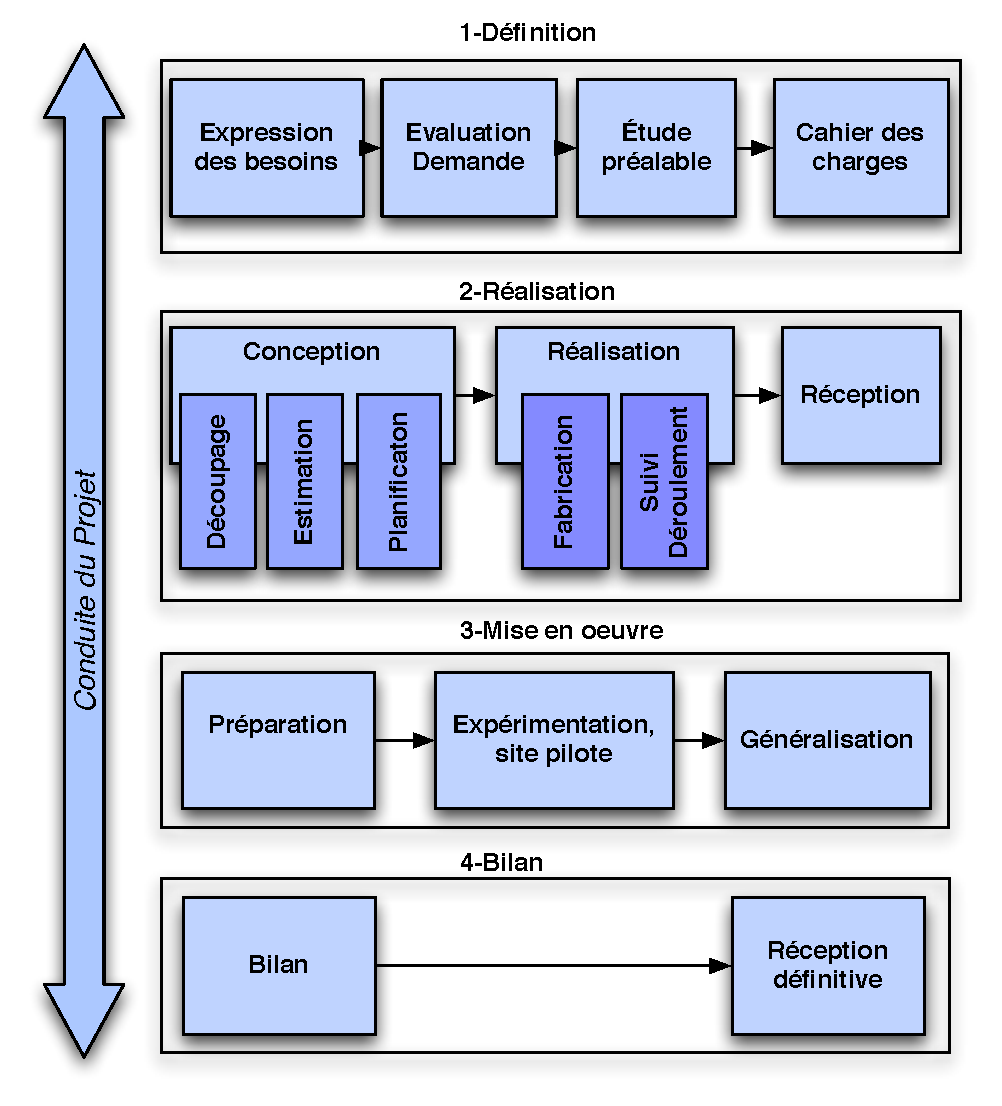
\includegraphics[height=\textheight]{overview-projet.pdf}
\end{center}
}

%*****************************************************************
\subsection{Assurer le lancement du projet: l'évaluation}

\frame{
\frametitle{Etude d'opportunité informelle}

\vspace{.5cm}
Avant acceptation ou lancement, se poser des questions :\\ 

\vspace{.5cm}
Toute difficulté identifiée devra faire l'objet 
d'un dialogue approfondi avec le demandeur pour

\begin{itemize}
\item soit annuler, infléchir ou différer le projet
\item soit négocier des moyens de réussite à hauteur des enjeux et des conditions de
réussite identifiées.
\end{itemize}

\vspace{.5cm}
$\Rightarrow$ Une \underline{évaluation} 
sous différents angles est nécessaire.
}

\frame{
\frametitle{Exemple simple: l'électricien}

\begin{block}{La demande}
Le client veut un site web pour 
\begin{itemize}
\item informer ses clients (horaires, produits, services, ...),
\item enregistrer demandes de devis, 
\item distribuer un dépliant electronique, 
\item ...
\end{itemize}
\end{block}
}

\frame{
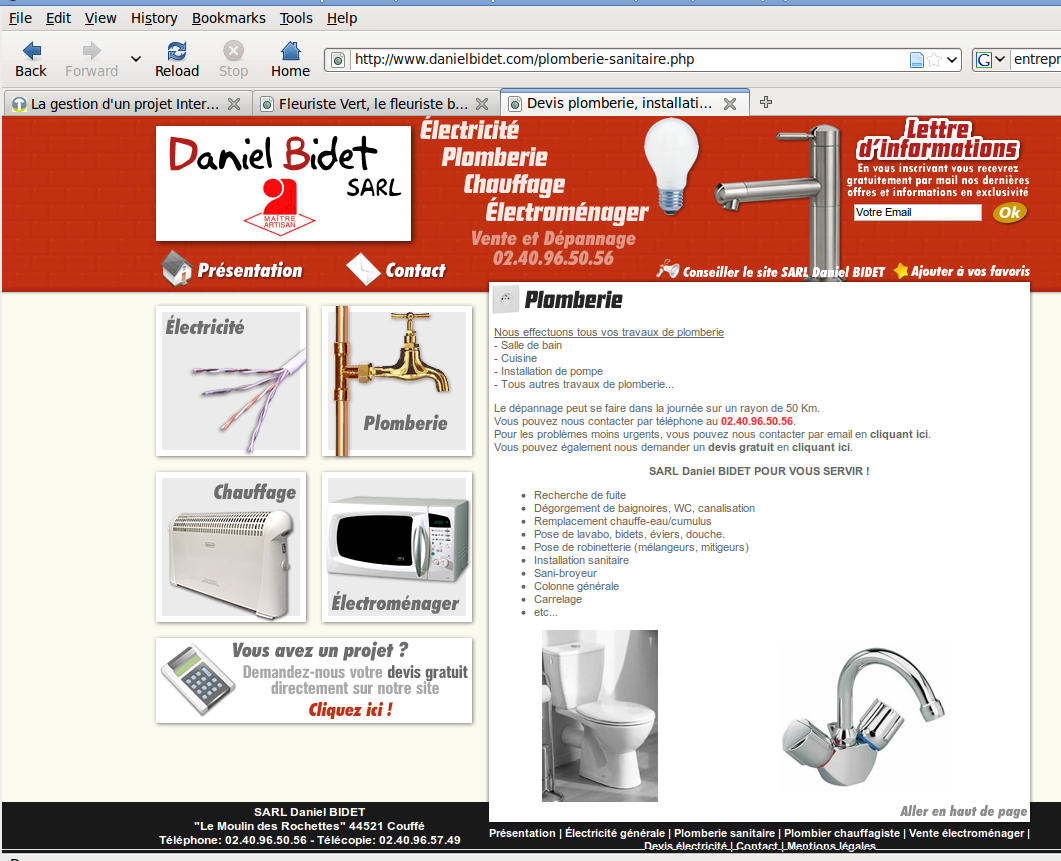
\includegraphics[width=\textwidth]{capture-site-electr.png}
}

\frame{
\frametitle{Exemple simple: l'électricien}

\begin{block}{La demande}
Le client veut un site web pour 
\begin{itemize}
\item informer ses clients (horaires, produits, services, ...),
\item enregistrer demandes de devis, 
\item distribuer un dépliant electronique, 
\item ...
\end{itemize}
\end{block}

\only<2>{Simple, non ? ...}
\only<3>{... Pourtant, répondre à cette demande nécessite de dialoguer avec le client.}

}
\frame{
\textit{
Quelques questions immédiates (liste non-exhaustive):
\begin{itemize}
    \item<+-> Qui décidera des informations nouvelles à enregistrer et publier ?
    \item<+-> Sur quels critères mettra t-on les informations produits/tarifs à jour ?
    \item<+-> De qui et comment viendront ces informations ?
    \item<+-> Qui mettra ces informations en ligne, sous quelle forme ? 
    \item<+-> Quelles compétences sont requises pour intervenir sur le site ? 
    \item<+-> Les visiteurs auront-ils le moyen d'enregistrer des alertes ? 
    \item<+-> Qui sera alerté ? Avec quels critères ? 
    \item<+-> ... Un deuxième niveau de questions devra cerner les motivations des acteurs...
\end{itemize}
}

\vspace{5mm}
\only<9>{Risque: un site au contenu périmé \ding{63} }
\only<10>{$\Rightarrow$ Adopter une démarche d'évaluation: le projet est-il clairement défini ?}
}

%*****************************************************************
\frame{
\frametitle{Evaluer le projet (1)}

Entre l'idée et sa réalisation, il peut y avoir un gouffre.
Le résultat attendu peut être flou et les implications mal cernées.  

\begin{block}{Règle 1 : Définissez l'idée en termes de résultat attendu}
    S'assurer que les décideurs sont d'accords avec ces résultats et peuvent dire ce qui va changer par rapport à ce qui est connu.

\pause
    \begin{itemize}
    \item<+-> Tous les acteurs ont ils la même représentation du produit attendu ?
    \item<+-> Cerner la demande : demande énoncée clairement, nature de la demande, cadre de la demande, les délais 
    \item<+-> Quels changements l'idée va t-elle produire ? Sont ils acceptables dans les structures et comportements ?
Que faut il faire pour les rendre acceptables ? 
    \end{itemize}
\end{block}  
}



\frame{
\frametitle{Evaluer le projet}

Le résultat attendu peut être ``contre-nature''.

\begin{block}{Règle 2 : évaluer la cohérence} 
Evaluer par la cohérence du projet dans le contexte de l'organisation
    \begin{itemize}
    \item<+-> Identifier le demandeur et protagonsites impliqués (initiateur, décideur, destinataire)
		% Ex: la demande vient des utilisateurs d'un service, relayée par le responsable du service,
		% appuyée par le chef du département et avalisée par la direction
    \item<+-> Générateur de résultats économiques ?
		% Va t-on avoir des gains ? quantifiables ?
    \item<+-> Les résultats escomptés sont ils en accord avec la stratégie de l'entreprise ? 
		% pas de contradiction avec les objectifs généraux affichés
		% Ex: l'entreprise annonce qu'elle passe d'une distrib. par revendeurs à distrib. directe mais le projet
		% concerne l'amélioration de la logistique de livraison des revendeurs
    \item<+-> Le projet s'inscrit-il dans la planification générale de l'entreprise ?
    Positionnement vis-à-vis d'autres projets ou actions ? (antinomies, synergies, compétition )
		% Ex: le projet logistique permet de livrer et d'informer les distributeurs sur les nouveaux produits mais
		% parallèlement un projet d'extranet revendeurs fournira également un catalogue et infos produits
    \end{itemize}
\end{block}
}


\frame{
\frametitle{Evaluer le projet }

Le projet peut devenir incontrôlable.

\begin{block}{Règle 3 : évaluer la conduite de projet} 
Evaluer par la conduite de projet : les risques d'aléas
    \begin{itemize}
    \item <+-> Garanties de progression et d'achèvement ? 
    \item <+-> Programme des étapes et décisions intermédiaires connus ?
    \item <+-> Les indicateurs de bonne fin sont ils précisés ?
    \end{itemize}
	
\end{block}
}

%******** CAS Personal Fit  ***************************
\frame{
\frametitle{Cas \textit{Personal Fit}}

\textbf{4.5.6} est une enseigne de prêt à porter pour femme, dont la cible est
la clientèle 30-50 ans. La marque est présente sous la forme d'un réseau de
franchisés (95 boutiques).

Elle désire lancer une offre distinctive \textit{Personal Fit}, un service de
vêtements ``sur mesure`'': une gamme spécifique de vêtements avec un choix de tailles
beaucoup plus fin, qui peut être guidé par des mesures electroniques. 

\vspace{5mm}
\begin{center}
\ldots voir étude de cas \ldots
\end{center}
}



%******************************************************************
\subsection{Le triangle projet: objectifs, délais, ressources}

\frame{
\frametitle{Le triangle projet}
 
\input{triangle.pdftex_t}

\vfill                 
}

%*****************************************************************
\frame{
\frametitle{Les objectifs}

\begin{center}
	`` Quoi faire ? ''
\end{center}
Définir le domaine couvert en termes de fonctionnalités. 
Le document contractuel est le \alert{cahier des charges}.
}

\frame{
\frametitle{Les délais}
\begin{center}
	`` Quand faire ? ''
\end{center}
La gestion des délais intervient une fois les étapes de découpage et d'estimation terminées. 
Un \alert{calendrier} contractuel définissant les délivrables intermédiaires peut être établi.
}

 
\frame{
\frametitle{Les ressources}

\begin{center}
	`` Avec qui/quoi faire ? ''
\end{center}


La gestion des ressources nécessite une \alert{organisation} parfois complexe.\\

Des structurations typiques des ressources humaines sont:
\begin{itemize}
\item structuration générale \emph{client/fournisseur}.
\item structuration en \emph{maîtrise d'ouvrage/maîtrise d'{\oe}uvre}.
\end{itemize}
}

\subsection{Structurations typiques pour les ressources humaines}
%******************************************************************
\frame{
\frametitle{Structuration client/fournisseur}

Dans de nombreux projets, on peut retrouver les acteurs suivants:

\underline{parmi les clients} :
\begin{itemize}
\item les décideurs
\item le chef de projet
\item les usagers
\end{itemize}

\underline{parmi les fournisseurs} :
\begin{itemize}
\item le chef de projet
\item les concepteurs
\item les équipes de fabrication
\end{itemize}
\vfill
}
%******************************************************************

\frame{
\frametitle{Structuration maîtrise d'ouvrage/maîtrise d'{\oe}uvre}

Quand les entreprises sont structurées pour gérer des projets 
on a souvent une organisation en \textbf{maîtrise d'ouvrage} (MOA) et
 \textbf{maîtrise d'{\oe}uvre} (MOE).\\

\pause
Ce sont deux entités de l'organisation (personnes morales).
\pause

\begin{itemize}
\item<+-> Le MOA est client du MOE à qui il passe commande d'un produit nécessaire à son activité.
\item<+-> Le MOE fournit ce produit: soit il le réalise lui-même, soit il passe commande à un ou plusieurs fournisseurs qui élaborent le produit sous sa direction. 
\end {itemize} 

}

\frame{
\frametitle{Les acteurs : structuration}
\input{acteurs.pdftex_t}

}   
\frame{
\frametitle{La maîtrise d'ouvrage : 6 fonctions}
\begin{itemize}
\item<+-> le maître d'ouvrage stratégique (MOAS)\\
	$\rightarrow$ prend les décisions, arbitre.
\item<+->  le maître d'ouvrage délégué (MOAD)\\
	$\rightarrow$ fournit les éléments factuels au MOAS.
\item<+->  le maître d'ouvrage opérationnel (MOAO)\\
	$\rightarrow$ expert d'un grand processus du métier.
\item<+->  l'assistant à maîtrise d'ouvrage (AMO),\\
      $\rightarrow$ support pour le MOAO ou MOAD en période de pointe, ou quand le projet demande des compétences non maitrisées. 
\item<+->  l'expert métier,\\
      $\rightarrow$ vérifie la pertinence du produit avec les exigences des utilisateurs
\item<+->   l'utilisateur\\
       $\rightarrow$ peuvent compléter les observations de l'expert métier.
\end {itemize}

}

\frame{
\frametitle{La maîtrise d'{\oe}uvre}

Le MOE est responsable de la qualité technique de la solution. 
Il doit, avant toute livraison au MOA, 
procéder aux vérifications nécessaires (``recette usine'').\\

\vspace{1cm}
 
Pour cela, le MOE doit assurer la coordination de tous les fabriquants en veillant (entre autres):
\begin{itemize}
\item à la cohérence des fournitures et à leur compatibilité,
\item à coordonner l'action des fournisseurs en contrôlant la qualité technique,
\item à respecter les délais fixés par le MOA et en minimisant les risques.
\end{itemize}
}

  
%*****************************************************************
\begin{comment}
\subsection{Eléments de motivation}
\frame{
\frametitle{Motiver l'équipe de projet}

Chaque acteur s'engagera d'autant plus que :
 
\begin{itemize}
\item le résultat de son action est visible
\item le résultat envisagé est désiré
\item sa confiance dans sa capacité à agir est grande
\end{itemize} 


Provoquer ces trois facteurs :
\begin{itemize}
\item s'accorder sur le chemin à parcourir
\item assurer la continuité du processus
\item faire adhérer les équipes
\item agir par la hiérarchie
\item investir en ressources humaines, temps, argent
\end{itemize} 
}
\end{comment}
